\section{Alpha Wave Analysis}
As mentioned in chapter \ref{ch:motivation} the sources are classified into four group according to a dominant frequency.
For the provided EEG datasets the sources would be classified as alpha waves, with frequencies between 8 and 13 Hz.
With the results from the main algorithm it would be interesting to see how the recovered sources and the provided measurements act in the frequency domain, when filtered to be in the range of the alpha wave.

For this comparison the dataset for subject 1, \texttt{S1\_OClean} and \texttt{S1\_CClean}, with open and closed eyes EEG measurements, will be used. 
Furthermore, it is expected to see that the closed-eyes dataset have a higher amplitude as it is expected that more brain activity occur when you closed your eyes \todo{reference eller noget? -L}.

\subsection{Setup}
To perform the filtering according to the alpha wave frequency range a bandpass Butterworth filter of order 5 with cutoff frequency $8$ Hz and $13$ Hz will be applied to the datasets and the recovered sources from the main algorithm. This will be done in the time domain. 
To see the filtering process the datasets and recovered sources will after the filtering be transform into the frequency domain. This will be done with the fast Fourier transform (FFT).

In figure \ref{fig:dft_1} only one source was investigated in both time and frequency domain. The source of interest was recovered from the closed-eyes dataset \texttt{S1\_CClean} dataset from time segment $15$. Furthermore, the system specification used to recover the source was $M=27$ and $k=14$.
\begin{figure}[H]
\centering
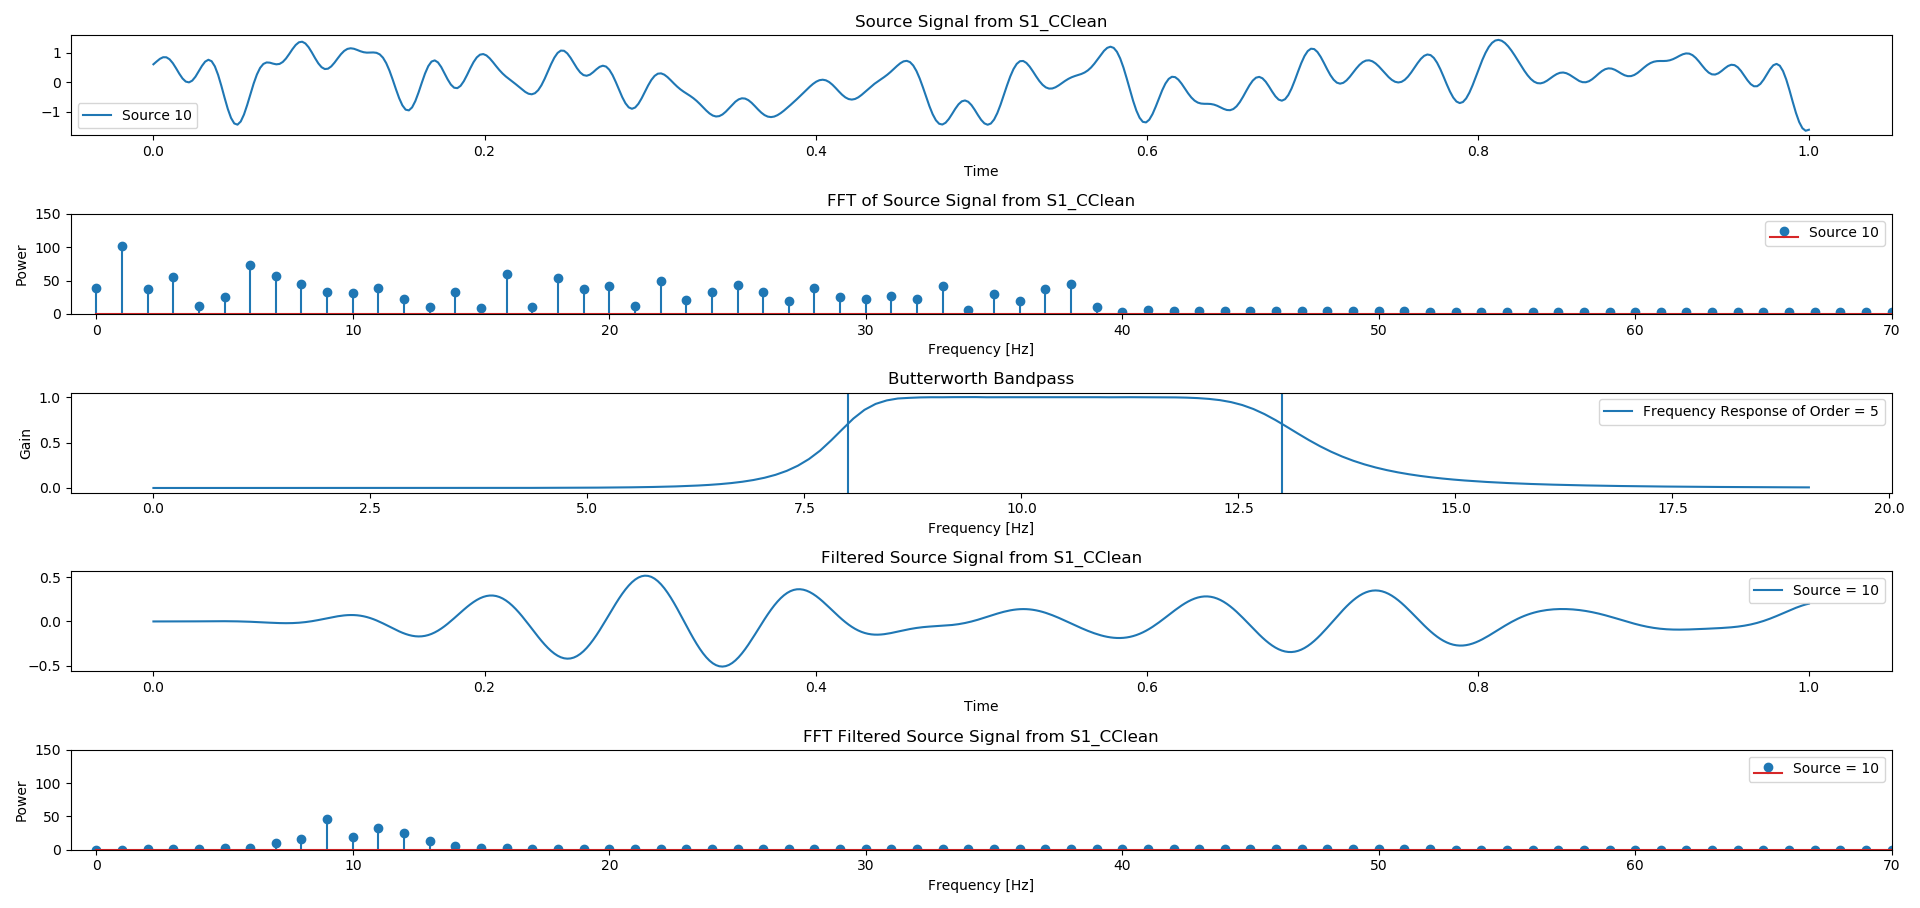
\includegraphics[scale=0.28]{figures/ch_7/DFT_plot_X_timeseg15_source10.png}
\caption{Time domain and frequency plot of a recovered source signal, filtered and non-filtered, from the time segment 15.}
\label{fig:dft_1}
\end{figure}
\noindent
The first plot in figure \ref{fig:dft_1} is the recovered source signal in the time domain. The next plot is the same source signal but transformed to the frequency domain with the FFT. The plot has been scaled to only show the frequencies from 0-70 Hz and the power from 0 to 150. The third plot illustrate the frequency response of the bandpass Butterworth filter with order 5. The vertical blue lines illustrate the cutoff frequency for 8 Hz and 13 Hz.
Plot number 4 is the recovered source signal filtered with the bandpass Butterworth filter which have been plot in the time domain. The last plot is the filtered source signal from plot 4 transformed to frequency domain, again with the FFT.

From the frequencies plot it can be seen that the signal of interest has been filtered according to the alpha wave. And from the filtered source signal in the time domain, the signal resemble the alpha wave as seen in figure \ref{fig:EEG_example}.

\subsection{Results}
The filtering process have been applied to the whole dataset of closed-eyes and open-eyes and the respectively recovered sources. Each time segment has been summed such that only one signal resemble each time segments.

Figure \ref{fig:dft_2} shows two filtered source signals and two filtered measurement signals, one from the open-eyes dataset \texttt{S1\_OClean} and one from the close-eyes dataset \texttt{S1\_CClean}, from the time segment 15.
\begin{figure}[H]
\centering
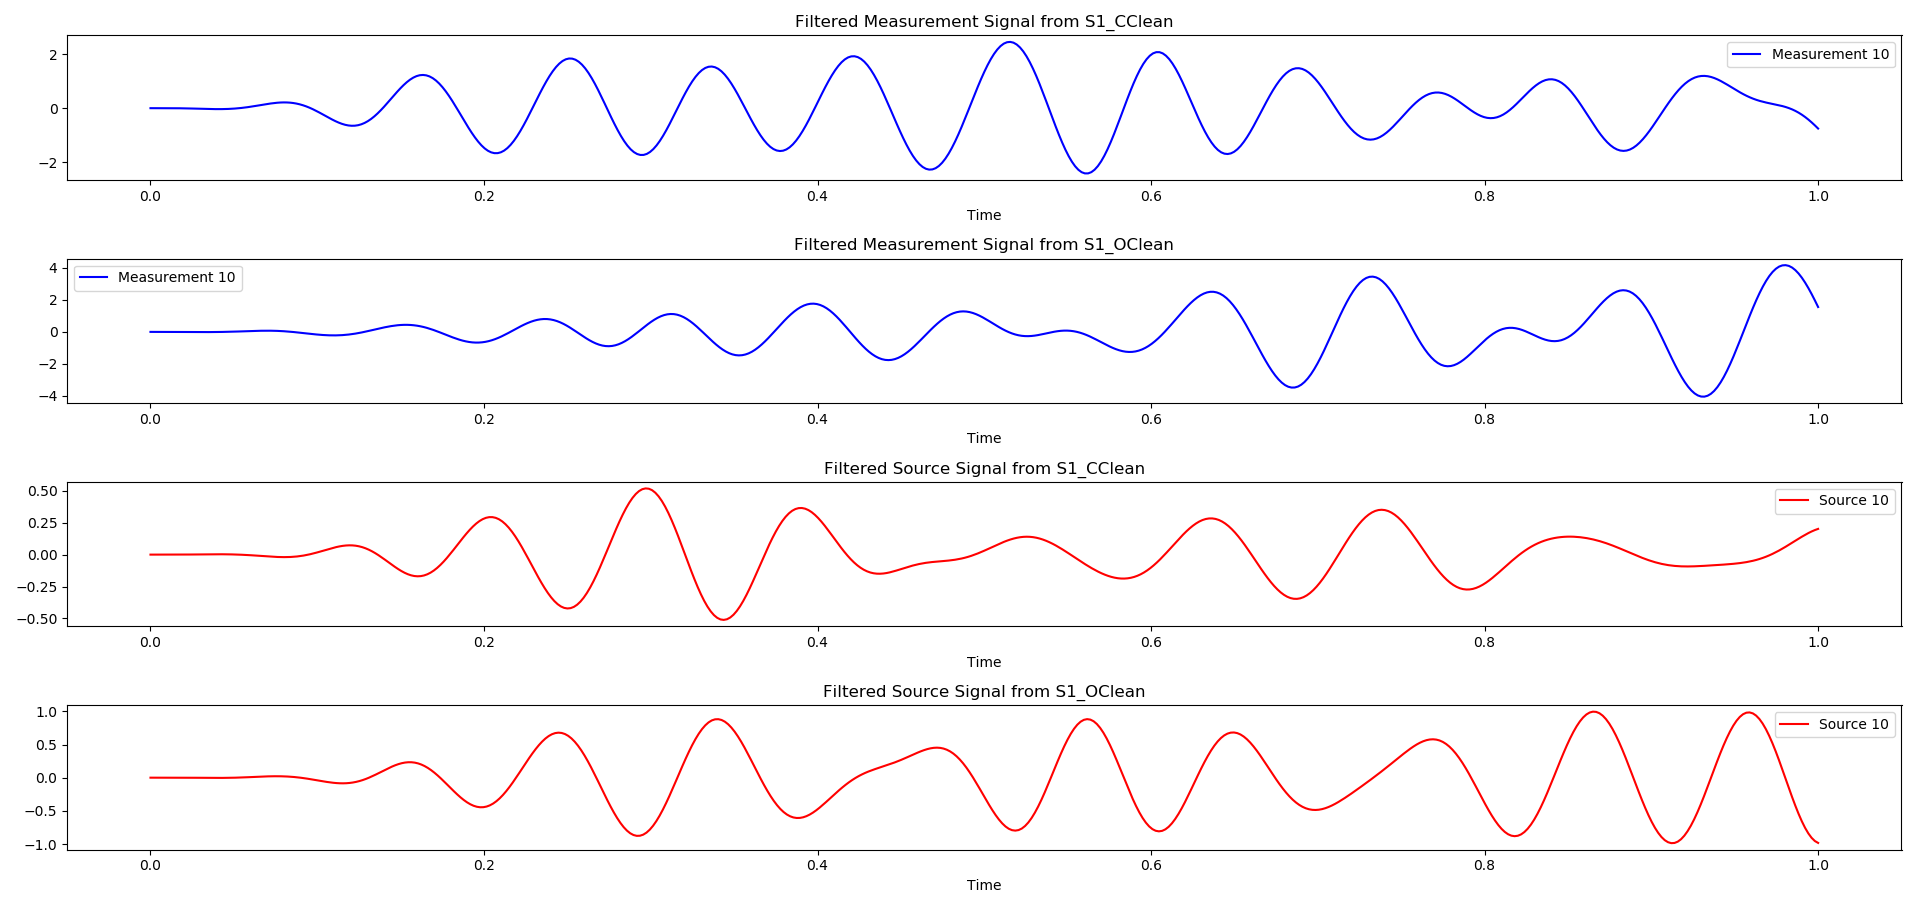
\includegraphics[scale=0.28]{figures/ch_7/DFT_plot_X_and_Y_signal_timeseg15_source10.png}
\caption{Filtered signals from measurement 10 and source 10 from time segment 15 from the closed eye dataset \texttt{S1\_CClean}.}
\label{fig:dft_2}
\end{figure}
\noindent
From figure \ref{fig:dft_2} it can be seen that a different between open-eyes and close-eyes datasets exists. From this example the difference from open-eyes to close-eyes measurement signals is $0.59$. The different from open-eyes to close-eyes source signals is $0.24$.
The close-eyes dataset for this example has a higher amplitude just as expected. 

Lets now investigate if this behaviour continues when looking at several signals. Figure \ref{fig:dft_3} is a sum of all signals in one time segment.
\begin{figure}[H]
\centering
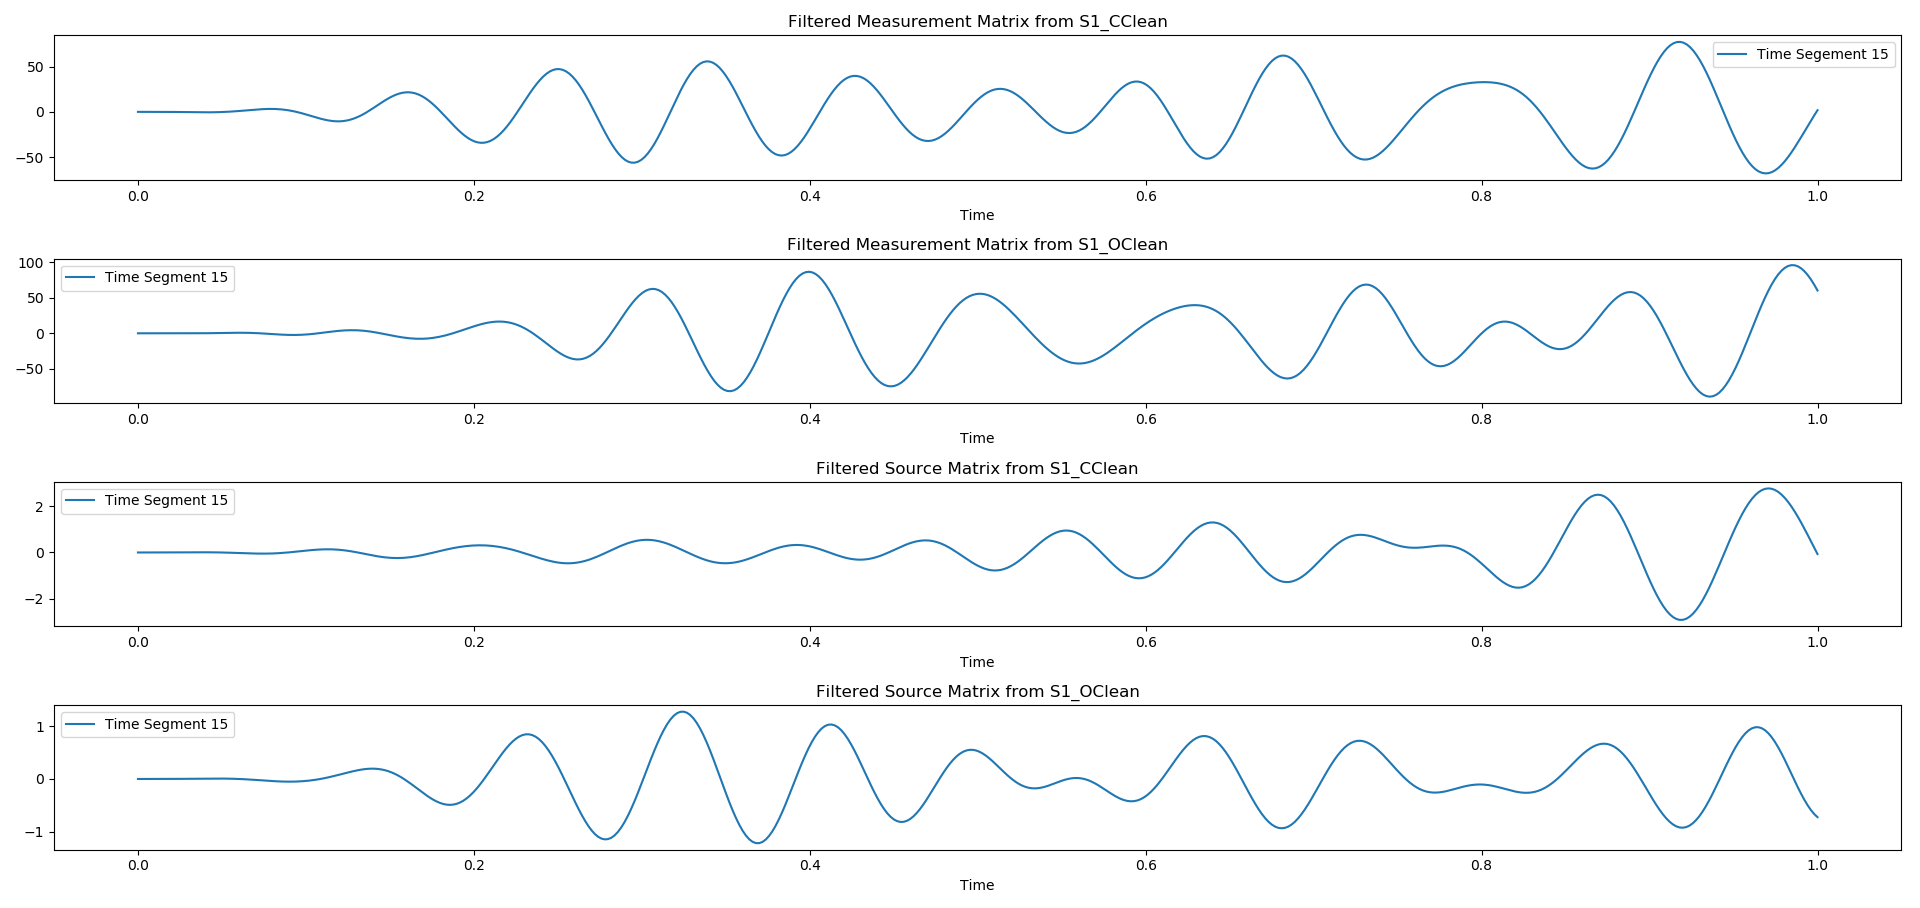
\includegraphics[scale=0.28]{figures/ch_7/DFT_plot_X_and_Y_matrix_timeseg15.png}
\caption{Filtered measurement matrix and source matrix for time segment 15. The rows of the matrices have been sum together.}
\label{fig:dft_3}
\end{figure}
\noindent
The difference from the open-eyes to close-eyes measurement signals is $1.99$. The different from open-eyes to close-eyes source signals is $0.43$. The same behaviour as seen in figure \ref{fig:dft_2} also occur in this case. Furthermore, the summed signals still resemble the alpha wave. 

Figure \ref{fig:dft_4} is figure \ref{fig:dft_3} transformed to the frequency domain with the FFT.
\begin{figure}[H]
\centering
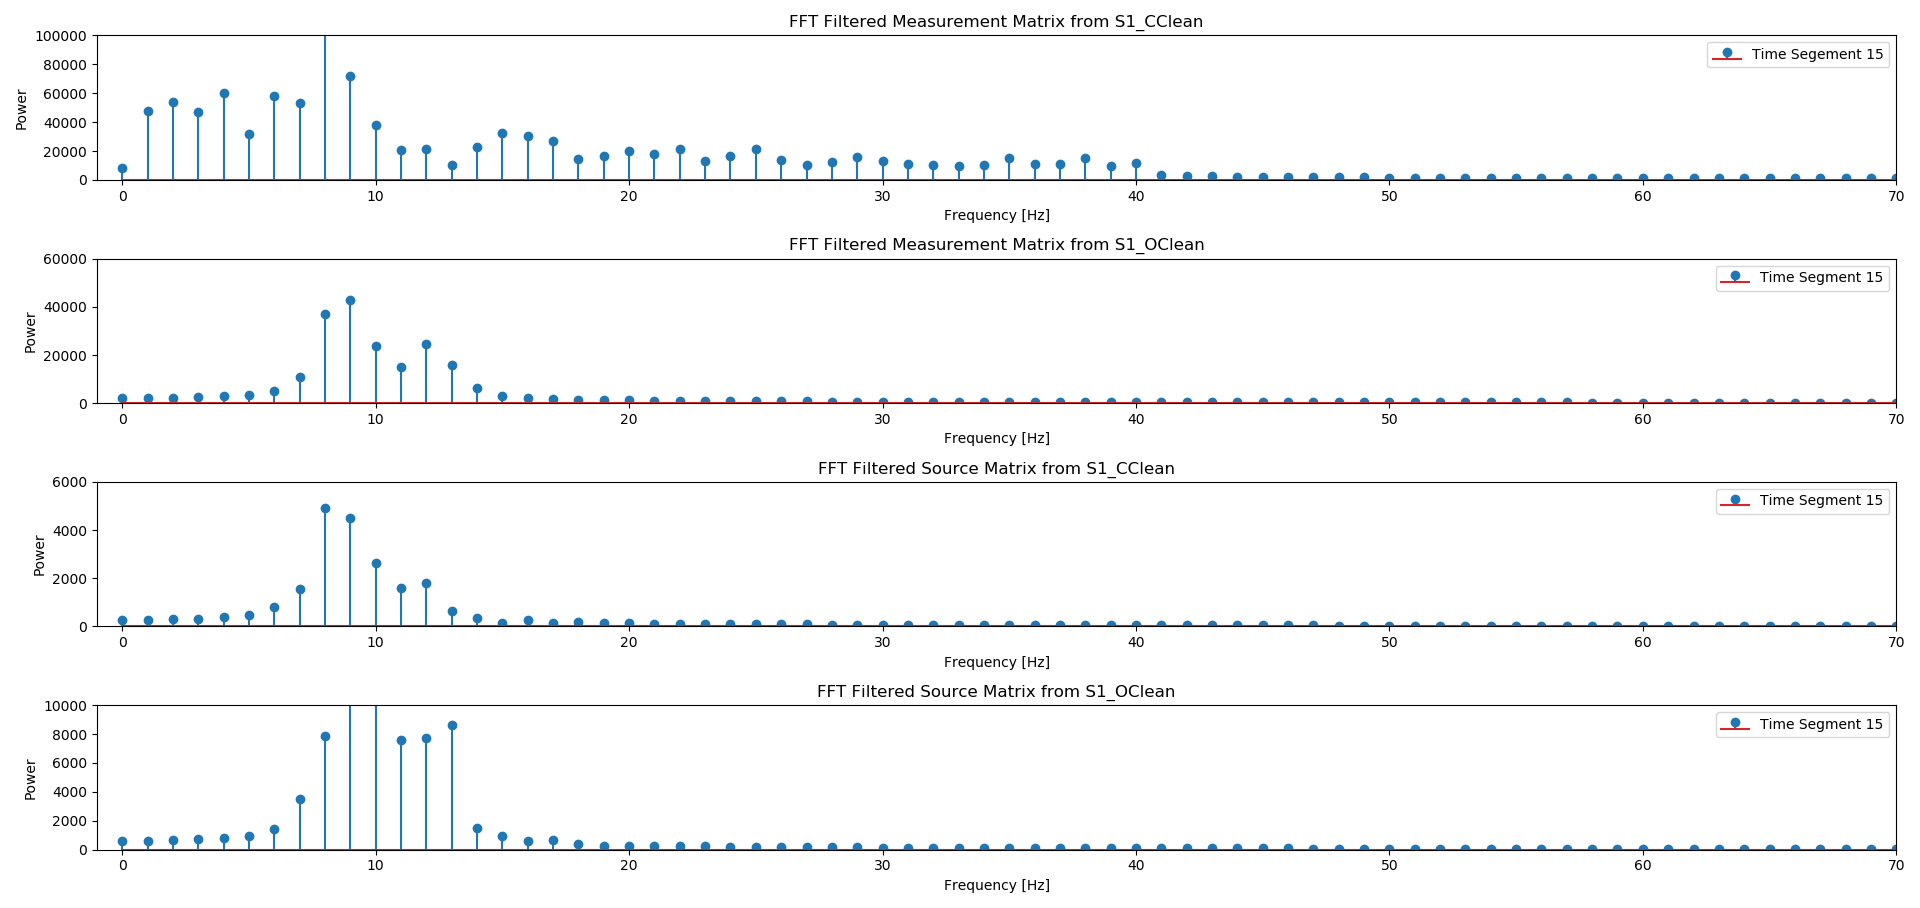
\includegraphics[scale=0.28]{figures/ch_7/DFT_plot_X_and_Y_matrix_timeseg15_power.png}
\caption{Filtered measurement matrix and source matrix for time segment 15. The rows of the matrices have been sum together.}
\label{fig:dft_4}
\end{figure}
\noindent
The following figure illustrate the difference between open-eyes to closed-eyes for 100 time segments.
\begin{figure}[H]
\begin{widepage}
    \begin{minipage}[t]{.49\textwidth}
\centering
\includegraphics[width=1\linewidth]{figures/ch_7/DFT_Y_Difference.png}
\caption{The average difference between the measurements of the open and closed eyes datasets for 100 time segments. The average difference total is $1.16$.}
\label{fig:dft_5}
\end{minipage} 
\hspace{.5cm}
\begin{minipage}[t]{.49\textwidth}
\centering
\includegraphics[width=1\linewidth]{figures/ch_7/DFT_X_Difference.png}
\caption{The average difference between the recovered sources of the open and closed eyes datasets for 100 time segments. The average difference total is $2.01$.}
	\label{fig:dft_6}
    \end{minipage}
\end{widepage}
\end{figure}
\noindent
From figure \ref{fig:dft_6} the overall difference between the recovered sources from the open-eyes dataset to the closed-eyes dataset is $2.01$ which support our expectation of the behaviour of brain activity. By the transformation according to the alpha wave frequency band the recovered sources behaves as expected and this support the that main algorithm recovers in some sense useful results.